\documentclass[12pt]{beamer}
\usepackage{../Estilos/BeamerMAF}
%Sección para el tema de beamer, con el theme, usercolortheme y sección de footers
\usetheme{CambridgeUS}
\usecolortheme{beaver}
%\useoutertheme{default}
\setbeamercovered{invisible}
% or whatever (possibly just delete it)
\setbeamertemplate{section in toc}[sections numbered]
\setbeamertemplate{subsection in toc}[subsections numbered]
\setbeamertemplate{subsection in toc}{\leavevmode\leftskip=3.2em\rlap{\hskip-2em\inserttocsectionnumber.\inserttocsubsectionnumber}\inserttocsubsection\par}
\setbeamercolor{section in toc}{fg=blue}
\setbeamercolor{subsection in toc}{fg=blue}
\setbeamercolor{frametitle}{fg=blue}
\setbeamertemplate{caption}[numbered]

\setbeamertemplate{footline}
\beamertemplatenavigationsymbolsempty
\setbeamertemplate{headline}{}


\makeatletter
\setbeamercolor{section in foot}{bg=gray!30, fg=black!90!orange}
\setbeamercolor{subsection in foot}{bg=blue!30!yellow, fg=red}
\setbeamercolor{date in foot}{bg=black, fg=white}
\setbeamertemplate{footline}
{
  \leavevmode%
  \hbox{%
  \begin{beamercolorbox}[wd=.333333\paperwidth,ht=2.25ex,dp=1ex,center]{section in foot}%
    \usebeamerfont{section in foot} \insertsection
  \end{beamercolorbox}%
  \begin{beamercolorbox}[wd=.333333\paperwidth,ht=2.25ex,dp=1ex,center]{subsection in foot}%
    \usebeamerfont{subsection in foot}  \insertsubsection
  \end{beamercolorbox}%
  \begin{beamercolorbox}[wd=.333333\paperwidth,ht=2.25ex,dp=1ex,right]{date in head/foot}%
    \usebeamerfont{date in head/foot} \insertshortdate{} \hspace*{2em}
    \insertframenumber{} / \inserttotalframenumber \hspace*{2ex} 
  \end{beamercolorbox}}%
  \vskip0pt%
}
\makeatother\newlength{\depthofsumsign}
\setlength{\depthofsumsign}{\depthof{$\sum$}}
\newcommand{\nsum}[1][1.4]{% only for \displaystyle
    \mathop{%
        \raisebox
            {-#1\depthofsumsign+1\depthofsumsign}
            {\scalebox
                {#1}
                {$\displaystyle\sum$}%
            }
    }
}
\def\scaleint#1{\vcenter{\hbox{\scaleto[3ex]{\displaystyle\int}{#1}}}}
\def\bs{\mkern-12mu}






\setbeamercolor{section in foot}{bg=atomictangerine, fg=white}
\setbeamercolor{subsection in foot}{bg=blue-violet, fg=white}
\setbeamercolor{date in foot}{bg=goldenrod, fg=white}

\makeatletter
\setbeamertemplate{footline}
{
  \leavevmode%
  \hbox{%
  \begin{beamercolorbox}[wd=.333333\paperwidth,ht=2.25ex,dp=1ex,center]{section in foot}%
    \usebeamerfont{section in foot} \insertsection
  \end{beamercolorbox}%
  \begin{beamercolorbox}[wd=.333333\paperwidth,ht=2.25ex,dp=1ex,center]{subsection in foot}%
    \usebeamerfont{subsection in foot}  \insertsubsection
  \end{beamercolorbox}%
  \begin{beamercolorbox}[wd=.333333\paperwidth,ht=2.25ex,dp=1ex,right]{date in head/foot}%
    \usebeamerfont{date in head/foot} \insertshortdate{} \hspace*{2em}
    \insertframenumber{} / \inserttotalframenumber \hspace*{2ex} 
  \end{beamercolorbox}}%
  \vskip0pt%
}
\makeatother

\usefonttheme{serif}
\resetcounteronoverlays{saveenumi}

\date{10 de marzo de 2022}

\title{\large{EDO con singularidades}}
\subtitle{Tema 2 - Método de Frobenius}
\author{M. en C. Gustavo Contreras Mayén}

\begin{document}
\maketitle
\fontsize{14}{14}\selectfont
\spanishdecimal{.}

\section*{Contenido}
\frame{\tableofcontents[currentsection, hideallsubsections]}

\section{El oscilador armónico cuántico}
\frame{\tableofcontents[currentsection, hideothersubsections]}
\subsection{Vibraciones en una molécula}

\begin{frame}
\frametitle{Vibraciones moleculares}
Los enlaces químicos en las moléculas no son rígidos al contrario están constantemente oscilando respecto a cierta posición de equilibrio.
\end{frame}
\begin{frame}
\frametitle{El oscilador cuántico}
El oscilador armónico cuántico explica la energía de vibración en las moléculas cuando las oscilaciones del enlace son pequeñas, lo que sucede a temperatura ambiente o si adicionamos energía a la molécula en forma de calor, la oscilación aumenta.
\end{frame}
\begin{frame}
\frametitle{El oscilador cuántico}
El modelo del oscilador armónico explica las oscilaciones o vibraciones de los enlaces químicos.
\\
\bigskip
\pause
Desde el punto de vista químico, esta vibración explica la existencia de los espectros de vibración.
\end{frame}

\subsection{La EDO del oscilador cuántico}

\begin{frame}
\frametitle{El oscilador cuántico}
El oscilador armónico cuántico está descrito mediante el Hamiltoniano:
\pause
\begin{align*}
- \dfrac{\hbar^{2}}{2 m} \, \dv[2]{\psi}{x} + \dfrac{m \, \omega^{2} \, x^{2}}{2} \, \psi = E \, \psi
\end{align*}
\end{frame}
\begin{frame}
\frametitle{Resultados esperados}
Con este ejercicio nos interesa encontrar:
\setbeamercolor{item projected}{bg=blue!70!black,fg=yellow}
\setbeamertemplate{enumerate items}[circle]
\begin{enumerate}[<+->]
\item El espectro de energía $E_{n}$
\item Las soluciones de esta ecuación diferencial $\psi_{n}$.
\end{enumerate}
\end{frame}
\begin{frame}
\frametitle{Simplificando la EDO}
Para facilitar el trabajo, construimos una variable adimensional, en la cual resolveremos la ecuación diferencial.
\end{frame}
\begin{frame}
\frametitle{EDO simplificada}
Dividimos el Hamiltoniano entre $\dfrac{2 \, m}{\hbar^{2}}$, para obtener:
\pause
\begin{eqnarray*}
\dv[2]{\psi}{x}  + \left( \dfrac{m \, \omega}{\hbar} \right)^{2} \, x^{2} \, \psi &=&  \dfrac{2 \, m \, E}{\hbar^{2}} \, \psi =  \\[0.5em] \pause
&=& \left( - \dfrac{2 \, E}{\hbar \, \omega} \right) \bigg( \dfrac{m \, \omega}{\hbar} \bigg) \, \psi
\end{eqnarray*}
\end{frame}
\begin{frame}
\frametitle{Otra simplificación}
Definimos la variable $\xi$ tal que:
\pause
\begin{align*}
\xi = \sqrt{\dfrac{m \, \omega}{\hbar}} \, x
\end{align*}
Revisemos que $\xi$ es una variable adimensional, permitiendo que la ecuación sea más sencilla de resolver.
\end{frame}
\begin{frame}
\frametitle{Avanzando en la simplificación}
Tomamos la derivada con respecto a $x$:
\pause
\begin{eqnarray*}
\begin{aligned}
\dv{x} &= \dv{\xi} \, \dv{\xi}{x} = \sqrt{\dfrac{m \, \omega}{\hbar}} \, \dv{\xi} \\[0.5em] \pause
\Longrightarrow \hspace{0.2cm} \dv[2]{x} &= \left( \dfrac{m \, \omega}{\hbar} \right) \, \dv[2]{\xi}
\end{aligned}
\end{eqnarray*}
\end{frame}
\begin{frame}
\frametitle{Avanzando en la simplificación}
Para llegar a lo siguiente:
\begin{align*}
\left( \dfrac{m \, \omega}{\hbar} \right) \, \dv[2]{\psi}{\xi} + \left( \dfrac{m \, \omega}{\hbar} \right) \left( \sqrt{\dfrac{m \, \omega}{\hbar}} \, x \right)^{2} \, \psi = \left( - \dfrac{2 \, E}{\hbar \, \omega} \right) \bigg( \dfrac{m \, \omega}{\hbar} \bigg) \, \psi
\end{align*}
\end{frame}
\begin{frame}
\frametitle{Otro paso en la simplificación}
Al multiplicar todo por $\hbar / (m \omega)$:
\pause
\begin{eqnarray*}
\dv[2]{\psi}{\xi} + \left( \sqrt{\dfrac{m \, \omega}{\hbar}} \, x \right)^{2} \, \psi &=& \left( - \dfrac{2 \, E}{\hbar \, \omega} \right) \, \psi = \\[0.5em] \pause
= \dv[2]{\xi} \psi + \xi^{2} \, \psi &=& - k \, \psi
\end{eqnarray*}
\pause
con $k = \dfrac{2 \, E}{\hbar \, \omega}$.
\end{frame}
\begin{frame}
\frametitle{LA EDO2H}
Se ha llevado la ecuación inicial a una expresión que corresponde a una EDO2H, que debemos de resolver:
\pause
\begin{align}
\dv[2]{\psi}{\xi} + \big( \xi^{2} - k \big) \, \psi = 0
\label{eq:ED_oscilador}
\end{align}
\end{frame}

\subsection{Singularidades}

\begin{frame}
\frametitle{Punto importante}
Recordemos que el método de Frobenius funciona si existen a lo más, singuralidades regulares en la ED, por lo que veamos cuáles y de qué tipo son las singularidades que presenta la EDO del oscilador armónico cuántico. 
\end{frame}
\begin{frame}
\frametitle{Puntos singulares en la EDO}
Si escribimos la EDO2H como:
\pause
\begin{align}
\sderivada{y} + P(x) \, \pderivada{y} + Q(x) \, y = 0
\label{eq:ecuacion_09_75}
\end{align}
\pause
Si las funciones $P(x)$ y $Q(x)$ permanecen finitas mientras $x \to x_{0}$, el punto $x = x_{0}$ es un \emph{punto ordinario}.
\par
\pause
Al contrario, si $P(x)$ y/o $Q(x)$ divergen mientras $x \to x_{0}$, el punto $x_{0}$ es un \emph{punto singular}.
\end{frame}
\begin{frame}
\frametitle{Puntos singulares en la EDO}
Usando la ecuación (\ref{eq:ecuacion_09_75}) podemos distinguir entre dos tipos de puntos singulares:
\pause
\setbeamercolor{item projected}{bg=blue!70!black,fg=yellow}
\setbeamertemplate{enumerate items}[circle]
\begin{enumerate}[<+->]
\item Si $P(x)$ y/o $Q(x)$ divergen a medida que $x \to x_{0}$, pero $(x - x_{0}) \: P(x)$ y $(x - x_{0})^{2} \: Q(x)$ permanecen finitas a medida que $x \to x_{0}$, entonces el punto $x = x_{0}$ se llama \textbf{punto singular regular o punto singular no esencial}.
\seti
\end{enumerate}
\end{frame}
\begin{frame}
\frametitle{Puntos singulares en la EDO}
\setbeamercolor{item projected}{bg=blue!70!black,fg=yellow}
\setbeamertemplate{enumerate items}[circle]
\begin{enumerate}[<+->]
\conti
\item Si $P(x)$ diverge más rápidamente que $\dfrac{1}{(x - x_{0})}$, de tal modo que $(x - x_{0}) \: P(x)$ tiene a infinito a medida que $x \to x_{0}$, o cuando $Q(x)$ diverge más rápidamente que $\dfrac{1}{(x - x_{0})^{2}}$, \pause de modo que $(x - x_{0})^{2} \: Q(x)$ tiene a infinito, a medida que $x \to x_{0}$, entonces el punto $x = x_{0}$ se llama \textbf{singularidad esencial o singularidad irregular}.
\end{enumerate}
\end{frame}
\begin{frame}
\frametitle{Las funciones $P(x)$ y $Q(x)$}
De la ecuación (\ref{eq:ED_oscilador}) se encuentra que:
\pause
\begin{align*}
P(x) = 0 \hspace{1cm} Q(x) = (\xi^{2} - k)
\end{align*}
\pause
Nos interesa estudiar los puntos $x = 0$ y $x \to \infty$.
\end{frame}
\begin{frame}
\frametitle{Puntos singulares}
De acuerdo a las definiciones anteriores, en la ec. (\ref{eq:ED_oscilador}), el punto $x = 0$ no es punto singular.
\\
\bigskip
\pause
Habrá que revisar cuando $x \to \infty$.
\end{frame}
\begin{frame}
\frametitle{Punto singular}
Se tiene que $(\xi^{2} - k)$ diverge más rápidamente que $\dfrac{1}{(\xi - \xi_{0})^{2}}$ cuando $\xi \to \infty$, de modo que:
\pause
\begin{align*}
(\xi - \xi_{0})^{2} \: Q(x) \to \infty
\end{align*}
a medida que $x \to x_{0}$.
\pause
\\
Por lo tanto: la EDO presenta un punto singular irregular \enquote{en el infinito}.
\end{frame}
\begin{frame}
\frametitle{Comportamiento de la EDO}
Cuando $\xi \to \infty$, el término dominante de la ec. (\ref{eq:ED_oscilador}) es $\xi^{2}$, por lo que la EDO a resolver es:
\pause
\begin{align}
\dv[2]{\psi}{\xi} +  \xi^{2} \, \psi = 0
\label{eq:ED_oscilador_infinito}
\end{align}
\end{frame}
\begin{frame}
\frametitle{Soluciones de la EDO}
Cuando $\xi \to \infty$ la ec. (\ref{eq:ED_oscilador_infinito}) tiene las soluciones:
\pause
\begin{align*}
\psi(\xi) = A \, \exp \left( - \dfrac{\xi^{2}}{2} \right) + B \, \exp \left( \dfrac{\xi^{2}}{2} \right) 
\end{align*}
\pause
En cumplimiento de los postulados de la mecánica cuántica, se requiere que $\psi(\xi)$ sea de tipo cuadrado integrable, \pause ya que de ésta manera, la función converge y se puede normalizar, \pause por tanto: $B = 0$.
\end{frame}
\begin{frame}
\frametitle{Aproximación a la solución}
Entonces la solución aproximada es:
\begin{align}
\setlength{\fboxsep}{3\fboxsep}\boxed{
\psi (\xi) \sim \exp \left( - \dfrac{\xi^{2}}{2} \right) \hspace{1cm} \mbox{ si } \xi \to \infty}
\end{align}
\end{frame}

\subsection{Solución propuesta}

\begin{frame}
\frametitle{Solución para desarrollar Frobenius}
Por lo revisado anteriormente, se propone la siguiente solución para la ec. (\ref{eq:ED_oscilador}):
\pause
\begin{align*}
\psi (\xi) = f (\xi) \, \exp \left( - a \, \xi^{2} \right) 
\end{align*}
\pause
La justificación de esta función de prueba es construir una función que converja.
\end{frame}
\begin{frame}
\frametitle{Solución para desarrollar Frobenius}    
Para ello removeremos el término $\xi^{2}$ mediante la función exponencial, posteriormente encontraremos la expansión en una serie de potencias de la función $f(\xi)$.
\end{frame}
\begin{frame}
\frametitle{Derivando la solución}
Se requiere obtener la primera y segunda derivada de $\psi(\xi)$, pero tenemos solo una función de manera explícita, mientras la $f(\xi)$ solo se indica.
\end{frame}
\begin{frame}
\frametitle{Regla de Leibinz}
Para obtener la derivada de orden $n$ de un producto de funciones $f(x)$ y $g(x)$, utilizamos la regla de Leibinz:
\pause
\begin{align*}
\dv[n]{x} f(x) \cdot g(x) = \nsum_{m=0}^{n} \binom{n}{m} \, \dv[n-m]{f(x)}{x}  \, \dv[m]{g(x)}{x}
\end{align*}
\end{frame}
\begin{frame}\frametitle{Las derivadas de $\psi$}
Se tiene entonces que:
\pause
\begin{eqnarray*}
\begin{aligned}
\psi &= f(\xi) \, e^{-a \xi^{2}} \\[0.5em] \pause
\pderivada{\psi} &= \pderivada{f}(\xi) \, e^{-a \xi^{2}} - 2 \, a \, \xi  \, e^{-a \xi^{2}} \, f(\xi) = \\[0.5em] \pause
&= e^{-a \xi^{2}} \big[ \pderivada{f}(\xi) -  2 \, a \, \xi \, f(\xi) \big] \\[0.5em] \pause
\sderivada{\psi} &= \sderivada{f}(\xi) \, e^{-a \xi^{2}} - 4 \, a \, e^{-a \xi^{2}} \, \pderivada{f}(\xi) \, \xi + f(\xi) \big[ 4 \, a^{2} \, \xi^{2} - 2 \, a \big] = \\[0.5em] \pause
&= e^{-a \xi^{2}} \big[ \sderivada{f}(\xi) - 4 \, a \, \pderivada{f}(\xi) \, \xi + f(\xi) (4 \, a^{2} \xi^{2} - 2 \, a) \big]
\end{aligned}
\end{eqnarray*}    
\end{frame}
\begin{frame}
\frametitle{Sustituyendo las expresiones}
Sustituyendo las expresiones anteriores en la ecuación de Schrödinger, tenemos que:
\pause
\begin{align*}
e^{-a \xi^{2}} \bigg[ &\sderivada{f}(\xi) - 4 \, a \, \pderivada{f}(\xi) \, \xi + f(\xi) (4 \, a^{2} \xi^{2} - 2 \, a) \bigg] + \\[0.5em]
&+ k \, e^{-a \xi^{2}} \, f(\xi) - \xi^{2} \, e^{-a \xi^{2}} \, f(\xi) = 0
\end{align*}
\end{frame}
\begin{frame}
\frametitle{Sustituyendo las expresiones}
Por lo que:
\pause
\begin{align*}
\sderivada{f}(\xi) &- 4 \, a \, \pderivada{f}(\xi) \, \xi + f(\xi) \big[ 4 \, a^{2} \xi^{2} - 2 \, a \big] + \\[0.5em]
&+ k \, f(\xi) - \xi^{2} \, f(\xi) = 0
\end{align*}
\end{frame}
\begin{frame}
\frametitle{Sustituyendo las expresiones}
Removemos los términos con potencias $\xi^{2}$:
\pause
\begin{align*}
\sderivada{f}(\xi) - 4 \, a \, \pderivada{f}(\xi) \, \xi + f(\xi) \big[ 4 \, a^{2} \xi^{2} - 2 \, a - \xi^{2} +  k \big] = 0
\end{align*}
\end{frame}
\begin{frame}
\frametitle{EDO obtenida}
Por tanto:
\pause
\begin{align*}
4 \, a^{2} \, \xi^{2} - \xi^{2} = 0 \hspace{0.2cm} \Longrightarrow \hspace{0.2cm} a = \dfrac{1}{2}
\end{align*}
\pause
\begin{align*}
\sderivada{f}(\xi) - 4 \, a \, \xi \, \pderivada{f}(\xi) + (k - 2 \, a) \, f(\xi) = 0
\end{align*}    
Se ha removido la singularidad en el infinito, ya que no aparece el término $\xi^{2}$.
\end{frame}
\begin{frame}
\frametitle{EDO con nombre}
La ecuación diferencial obtenida luego del desarrollo es:
\pause
\begin{align*}
\addtolength{\fboxsep}{5pt}\boxed{
\sderivada{f} (\xi) - 2 \, \xi \, \pderivada{f}(\xi) + (k - 1) \, f(\xi) = 0}
\end{align*}
A esta ecuación se le conoce como la \emph{ecuación diferencial de Hermite}.
\pause
\\
\par
El siguiente paso es resolver la EDO de Hermite mediante una serie de potencias.
\end{frame}

\section{Solución por Frobenius}
\frame{\tableofcontents[currentsection, hideothersubsections]}
\subsection{Solución propuesta}

\begin{frame}
\frametitle{Solución propuesta para el desarrollo}
Consideremos la siguiente solución:
\pause
\begin{align*}
f(\xi) = \nsum_{n=0}^{\infty} a_{n} \, \xi^{n+r}
\end{align*}
\pause
Se propone esta solución ya que la ecuación de Hermite no posee singularidades en el infinito.
\end{frame}
\begin{frame}
\frametitle{Diferenciando la solución}
Entonces diferenciamos la solución en dos ocasiones:
\pause
\begin{align*}
\pderivada{f}(\xi) &= \nsum_{n=0}^{\infty} (n {+} r) \, a_{n} \, \xi^{n+r-1} \\[0.5em]
\sderivada{f}(\xi) &= \nsum_{n=0}^{\infty} (n {+} r)(n {+} r {-} 1) a_{n} \,  \xi^{n+r-2} 
\end{align*}
\end{frame}
\begin{frame}
\frametitle{Sustituyendo en la EDO}
Entonces al sustituir en la ecuación diferencial:
\pause
\begin{align*}
&\nsum_{n=0}^{\infty} (n {+} r) \, (n {+} r {-} 1) \, a_{n} \, \xi^{n+r-2} - 2 \, \xi \, \nsum_{n=0}^{\infty} (n {+} r) \, a_{n} \,  \xi^{n+r-1} + \\[0.3em]
&+ (k {-} 1) \nsum_{n=0}^{\infty} a_{n} \, \xi^{n+r} = 0
\end{align*}
\end{frame}
\begin{frame}
\frametitle{Sustituyendo en la EDO}
Reducimos el exponente en la segunda suma:
\pause
\begin{align*}
&\nsum_{n=0}^{\infty} (n {+} r) \, (n {+} r {-} 1) \, a_{n} \,  \xi^{n+r-2} - 2 \, \nsum_{n=0}^{\infty} (n {+} r) \, a_{n} \,  \xi^{n+r} + \\[0.3em]
&+ (k {-} 1) \nsum_{n=0}^{\infty} a_{n} \, \xi^{n+r} = 0
\end{align*}    
\end{frame}
\begin{frame}
\frametitle{Expresión obtenida}
Factorizando los términos para $\xi^{n+r}$:
\pause
\begin{align*}
&\nsum_{n=0}^{\infty} (n {+} r) \, (n {+} r {-} 1) \, a_{n}  \, \xi^{n+r-2} + \\[0.5em] 
&+ \nsum_{n=0}^{\infty} \bigg[ (k {-} 1) {-} 2 \, (n {+} r) \bigg] \, a_{n} \,  \xi^{n+r}  = 0
\end{align*}
\end{frame}
\begin{frame}
\frametitle{Términos de la primera suma}
En la primera suma, los términos para $n = 0, 1$, que corresponden a $\xi^{r-2}$ y $\xi^{r-1}$, están desapareados, \pause es decir, no existen términos con estos exponentes en la segunda suma.
\\
\bigskip
\pause
Por lo que deben de ser cero, para que $f(\xi)$ sea solución a la EDO.
\end{frame}
\begin{frame}
\frametitle{Casos para las raíces}
Se tiene entonces que:
\pause
\begin{align*}
a_{0} \, r \, (r - 1) &= 0 \\[0.5em]
a_{1} \, r \, (r + 1) &= 0
\end{align*}
\pause
Que tiene por única solución: $r = 0$.
\end{frame}
\begin{frame}
\frametitle{Reescribiendo la EDO}
La EDO se escribe como:
\pause
\begin{align*}
&\nsum_{n=0}^{\infty} n \, (n {-} 1) \, a_{n}  \, \xi^{n-2} + \\[0.5em] 
&+ \nsum_{n=0}^{\infty} \bigg[ (k {-} 1) {-} 2 \, n \bigg] \, a_{n} \, \xi^{n} = 0
\end{align*}
\end{frame}
\begin{frame}
\frametitle{De la primera suma}
Revisando la primera suma:
\pause
\begin{align*}
&\nsum_{n=0}^{\infty} n \, (n {-} 1) \, a_{n}  \, \xi^{n-2} = \nsum_{n=2}^{\infty} n (n {-} 1) \, a_{n} \, \xi^{n-2}        
\end{align*}
ya que para $n = 0, 1$, no se aporta nada en la suma.
\end{frame}
\begin{frame}
\frametitle{La expresión con los índices}
Se tiene que la suma es:
\pause
\begin{align*}
\nsum_{n=2}^{\infty} n (n {-} 1) \, a_{n} \, \xi^{n-2} + \nsum_{n=0}^{\infty} \bigg[ (k {-} 1) {-} 2 \, n \bigg] \, a_{n} \, \xi^{n} = 0
\end{align*}
\pause
Para manejar las dos sumas, deben de tener el mismo índice y el mismo exponente en $\xi$.
\end{frame}
\begin{frame}
\frametitle{Ajustando los índices}
Al ocupar la propiedad de las sumas:
\pause
\begin{align*}
\nsum_{n=0}^{\infty} (n {+} 2)(n {+} 1) \, a_{n+2} \, \xi^{n} + \nsum_{n=0}^{\infty} \bigg[ (k {-} 1) {-} 2 \, n \bigg] \, a_{n} \, \xi^{n} = 0
\end{align*}
\pause
Al tener el mismo índice y el exponente en las sumas, podemos agruparlas.
\end{frame}
\begin{frame}
\frametitle{Expresión para la suma}
\begin{align*}
\nsum_{n=0}^{\infty} \bigg[ (n {+} 2)(n {+} 1) \, a_{n+2} + \big( (k {-} 1) {-} 2 \, n \big) \,a_{n} \bigg] \, \xi^{n} = 0
\end{align*}    
\end{frame}
\begin{frame}
\frametitle{Condición en las sumas infinitas}
Para que la suma anterior se cumpla, todos los coeficientes de la serie deben de anularse, \pause por lo que conseguimos la relación de recurrencia:
\begin{align*}
\setlength{\fboxsep}{3\fboxsep}\boxed{
a_{n+2} = \dfrac{2 \, n + 1 - k}{(n + 2)(n + 1)} \, a_{n} }
\end{align*}
\end{frame}

\subsection{Espectro de energías}

\begin{frame}
\frametitle{Espectro de energías}
De la relación de recurrencia, para valores tales que $n \to \infty$, se tiene que:
\pause
\begin{align*}
a_{n+2} \approx \dfrac{2}{n} \, a_{n}
\end{align*}
\pause
por lo que la serie converge, ya que:
\pause
\begin{align*}
\displaystyle{\lim_{n \to \infty}} \dfrac{a_{n+2}}{a_{n}} = 0
\end{align*}
\end{frame}
\begin{frame}
\frametitle{Ocupando una serie}
Considerando la siguiente serie:
\pause
\begin{align*}
\exp \left( 2 \, \xi^{2} \right) = \nsum_{n=0}^{\infty} \dfrac{\left( 2 \, \xi^{2} \right)^{n}}{n!} = \nsum_{n=0}^{\infty} \dfrac{2^{n} \, \xi^{2n}}{n!}
\end{align*}
vemos que para esta serie:
\begin{align*}
\dfrac{a_{n+2}}{a_{n}} \approx \dfrac{2}{n}
\end{align*}
\end{frame}
\begin{frame}
\frametitle{Comparando series}
Lo que nos permite comparar la serie de $f(\xi)$ con $\exp( 2 \, \xi^{2})$.
\pause
\\
\bigskip
Es decir:
\begin{align*}
f(\xi) \approx \exp \left( 2 \, \xi^{2} \right) \hspace{1cm} \mbox{para $\xi$ grande}
\end{align*}
\end{frame}
\begin{frame}
\frametitle{Aproximación de la solución}
Tenemos que para $n \to \infty$ la solución se aproxima a:
\pause
\begin{align*}
\psi(\xi) \approx \exp \left( 2 \, \xi^{2}  \right) \, \exp \left( - \dfrac{\xi^{2}}{2} \right)
\end{align*}
\pause
pero esta solución diverge, por lo tanto no corresponde a una solución física real.
\end{frame}
\begin{frame}
\frametitle{Ajustando la expresión}
La solución física que mantiene la congruencia, es aquella donde la serie de potencias se trunca en algún punto.
\\
\bigskip
\pause
Es decir, que exista un valor $m$ tal que $a_{m+2} = 0$, de este modo, $f(\xi)$ pasa a ser un polinomio, \pause por tanto $f(\xi) \to 0$ cuando $\xi \to \infty$.
\end{frame}
\begin{frame}
\frametitle{Regresamos a la relación de recurrencia}
Al establecer esta condición en la regla de recurrencia:
\pause
\begin{eqnarray*}
2 \, m + 1 - k &=& 0 \\[0.5em] \pause
\Rightarrow \hspace{0.3cm} k &=& 2 \, m + 1
\end{eqnarray*}
\pause
y del valor que se estableció para $k$ al inicio:
\pause
\begin{align*}
\setlength{\fboxsep}{3\fboxsep}\boxed{
E = \hbar \, \omega \, \left( m + \dfrac{1}{2} \right) \hspace{1.5cm} m = 0, 1, 2, \ldots }
\end{align*}
\end{frame}

\subsection{Funciones de onda}

\begin{frame}
\frametitle{Usando el valor de $k$}
La relación de recurrencia puede escribirse nuevamente ocupando el valor encontrado de $k$:
\pause
\begin{align*}
a_{n+2} = \dfrac{-2 \, (m {-} n)}{(n {+} 2)(n {+} 1)} \, a_{n}
\end{align*}
\end{frame}
\begin{frame}
\frametitle{Paridad en los coeficientes}
Se tiene una relación entre los coeficientes de la misma paridad, es decir:
\begin{align*}
a_{0}, a_{2}, a_{4}, \ldots \hspace{0.5cm}
a_{1}, a_{3}, a_{5}, \ldots
\end{align*}
\pause
Por lo que podemos escribir a $f(\xi)$ como:
\pause
\begin{align*}
f(\xi) = f_{\mbox{par}} (\xi) + f_{\mbox{impar}} (\xi)
\end{align*}
\end{frame}
\begin{frame}
\frametitle{Paridad de los coeficientes}
La solución par depende de $a_{0}$:
\pause
\begin{align*}
f_{\mbox{par}} (\xi) \equiv a_{0} + a_{2} \, \xi^{2} + a_{4} \, \xi^{4} + \cdots
\end{align*}
\pause
Mientras que la impar depende de $a_{1}$:
\pause
\begin{align*}
f_{\mbox{impar}} (\xi) \equiv a_{1} \, \xi + a_{3} \, \xi^{3} + a_{5} \, \xi^{5} + \cdots
\end{align*}
\end{frame}
\begin{frame}
\frametitle{Normalizando la solución}
Se espera que la solución sea normalizable, por lo que:
\setbeamercolor{item projected}{bg=blue!70!black,fg=yellow}
\setbeamertemplate{enumerate items}[circle]
\begin{enumerate}[<+->]
\item Si $m$ es par, entonces $a_{1} = 0$.
\item Si $m$ es impar, entonces $a_{0} = 0$.
\end{enumerate}
\pause
La solución de paridad opuesta a $m$ se debe de cancelar, ya que de lo contrario, la solución diverge y $f(\xi)$ no sería la solución física del problema.
\end{frame}
\begin{frame}
\frametitle{Calculando algunos valores}
\begin{eqnarray*}
n = 0 \pause \rightarrow a_{1} = 0 \pause \Rightarrow f(\xi) = a_{0} \pause \Rightarrow \textcolor{red}{\psi_{0}(\xi) = a_{0} \exp \left( - \dfrac{\xi^{2}}{2} \right)}
\end{eqnarray*}
\pause
\begin{figure}
    \centering
    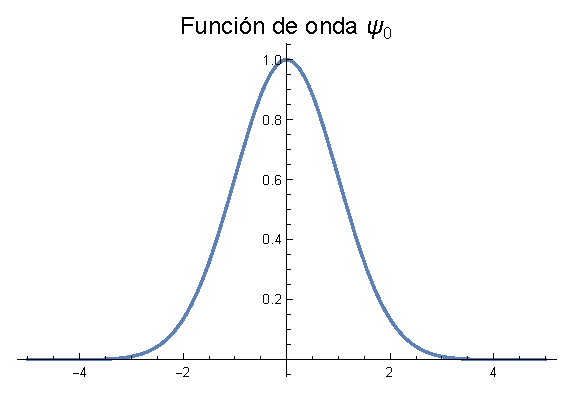
\includegraphics[scale=0.7]{Imagenes/Funcion_Onda_Psi_0.eps}
\end{figure}
\end{frame}
\begin{frame}
\frametitle{Calculando algunos valores}
\begin{eqnarray*}
n &= 1 \pause \rightarrow a_{0} = 0 \pause \Rightarrow f(\xi) = a_{1} \xi \pause \Rightarrow \textcolor{red}{\psi_{1}(\xi) = a_{1} \xi \exp \left( - \dfrac{\xi^{2}}{2} \right)}
\end{eqnarray*}
\pause
\begin{figure}
    \centering
    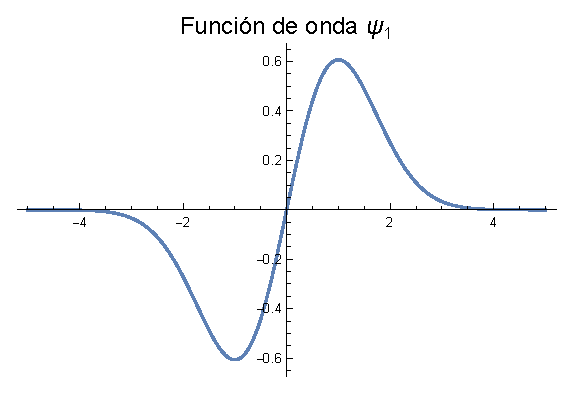
\includegraphics[scale=0.65]{Imagenes/Funcion_Onda_Psi_1.eps}
\end{figure}
\end{frame}
\begin{frame}
\frametitle{Calculando algunos valores}
\begin{eqnarray*}
n &= 2 \pause \rightarrow a_{1} = 0 \pause \Rightarrow f(\xi) = a_{0} \left( 1 - 2 \xi^{2} \right) \pause \Rightarrow \\[0.5em]
&\Rightarrow \textcolor{red}{\psi_{2}(\xi) = a_{0} \xi \left( 1 - 2 \xi^{2} \right) \exp \left( - \dfrac{\xi^{2}}{2} \right)}
\end{eqnarray*}
\end{frame}
\begin{frame}
\frametitle{Gráfica de $\psi_{2}$}
\begin{figure}
    \centering
    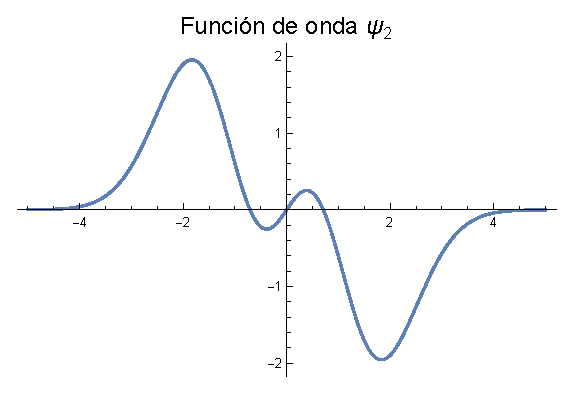
\includegraphics[scale=1]{Imagenes/Funcion_Onda_Psi_2.eps}
\end{figure}
\end{frame}
\begin{frame}
\frametitle{El método continua}
Podemos obtener otras funciones de onda de esta manera, \pause pero vemos que no sería nada práctico si quisiéramos conocer $\psi_{100}(\xi)$, para ello hay otro camino más sencillo.
\\
\bigskip
\pause
Cabe aclarar que las soluciones aún no están normalizadas.
\end{frame}
\begin{frame}
\frametitle{Uso de una función especial}
Consideremos a los polinomios de Hermite:
\pause
\begin{align*}
H_{0}(\xi) &= 1 \\[0.5em]
H_{1}(\xi) &= 2 \, \xi \\[0.5em]
H_{2}(\xi) &= 4 \, \xi^{2} - 2 \\[0.5em]
H_{3}(\xi) &= 8 \, \xi^{3} - 12 \, \xi \\[0.5em]
\vdots
\end{align*}
\end{frame}
\begin{frame}
\frametitle{Recuperando los polinomios de Hermite}
Los polinomios de Hermite forman parte del conjunto de funciones especiales que veremos en el Tema 5.
\\
\bigskip
\pause
Cada función especial se construye con ciertas características y propiedades, una de ellas es la fórmula de Rodrigues.
\end{frame}
\begin{frame}
\frametitle{Fórmula de Rodrigues para $H_{n}(\xi)$}
La fórmula de Rodrigues para los polinomios de Hermite es:
\begin{align*}
H_{n} (\xi) = (-1)^{n} \, \exp \left( \xi^{2} \right) \left( \dv{\xi} \right)^{n} \, \exp \left( - \xi^{2} \right)
\end{align*}
\end{frame}
\begin{frame}
\frametitle{Otra propiedad de los $H_{n}(\xi)$}
Las funciones especiales cuentan con una condición llamada de ortogonalidad:
\begin{align*}
\scaleint{5ex}_{\bs - \infty}^{\infty} H_{n}(\xi) \, H_{m}(\xi) \, \exp \left( - \xi^{2} \right) = \delta_{nm} \, \sqrt{\pi} \, 2^{n} \, n!
\end{align*}
\end{frame}
\begin{frame}
\frametitle{Solución al problema}
Con las propiedades de los polinomios de Hermite, los estados estacionarios del oscilador armónico cuántico son:
\begin{align*}
\setlength{\fboxsep}{3\fboxsep}\boxed{
\psi_{m}(\xi) = \left( \dfrac{m \omega}{\pi \hbar} \right)^{\frac{1}{2}} \dfrac{1}{\sqrt{2^{n} n!}} H_{m}(\xi) \exp \left( - \xi^{2} \right) }
\end{align*}
con:
\begin{align*}
\xi = \sqrt{\dfrac{m \omega}{\hbar}} \, x
\end{align*}
\end{frame}
\begin{frame}
\frametitle{Función de onda normalizada}
Con el uso de los polinomios de Hermite y sus propiedades, podemos obtener las funciones de onda $\psi_{n} (\xi)$ normalizadas.
\\
\bigskip
\pause
La tarea de resolver las integrales correspondientes implica dedicarle un buen rato, pero el resultado se obtiene y conviene graficar las soluciones normalizadas.
\end{frame}
\begin{frame}
\frametitle{Función de onda normalizada}
\begin{figure}
    \centering
    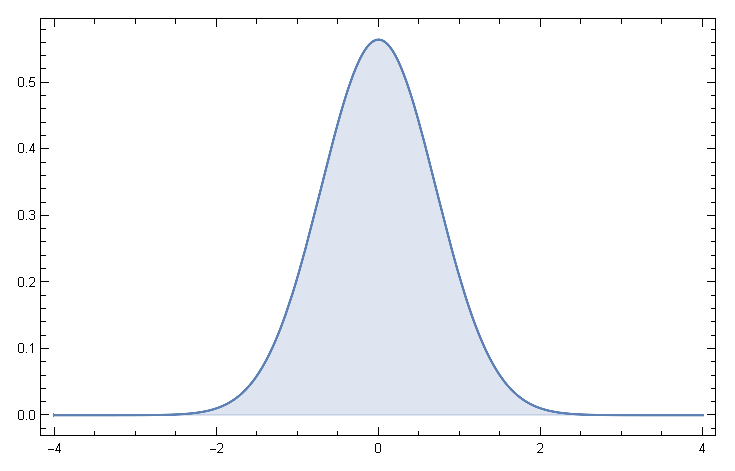
\includegraphics[scale=0.75]{Imagenes/Funcion_Onda_Normalizada_Psi_0.eps}
\end{figure}
\end{frame}
\begin{frame}
\frametitle{Función de onda normalizada}
\begin{figure}
    \centering
    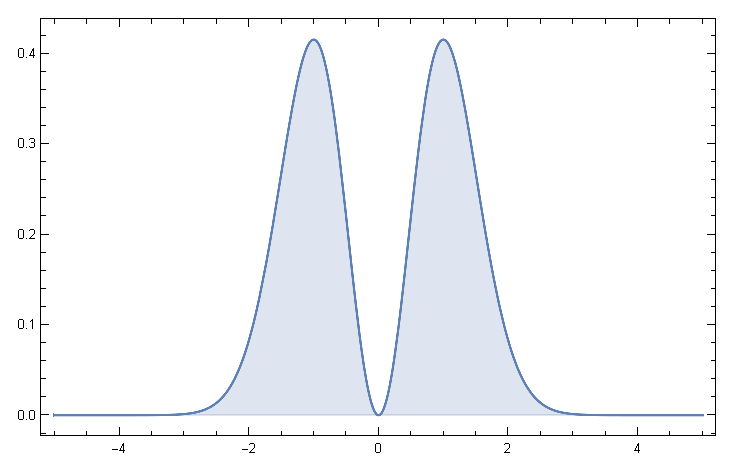
\includegraphics[scale=0.75]{Imagenes/Funcion_Onda_Normalizada_Psi_1.eps}
\end{figure}
\end{frame}
\begin{frame}
\frametitle{Función de onda normalizada}
\begin{figure}
    \centering
    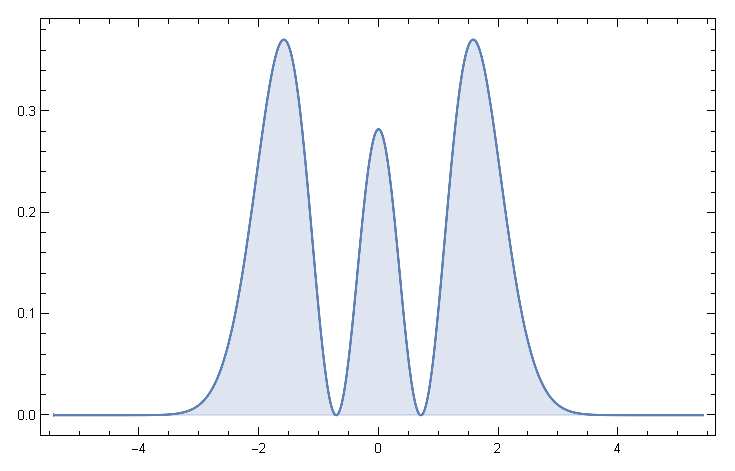
\includegraphics[scale=0.75]{Imagenes/Funcion_Onda_Normalizada_Psi_2.eps}
\end{figure}
\end{frame}
\begin{frame}
\frametitle{Pendiente por trabajar}
Para aceptar la solución al problema del oscilador armónico cuántico, se requiere demostrar que los polinomios de Hermite forman una base completa.
\\
\bigskip
Esto es lo que veremos en el Tema 3 del curso.
\end{frame}
\end{document} 